\chapter{RFID Systems}
In this chapter we explore the anatomy of an RFID system: its components, typical characteristics and common applications. We then dive into the Medium Access Control (MAC) problem that arises when many passive tags respond to a reader, review the families of solutions that were proposed.

\begin{redbar}
\textbf{Radio-Frequency Identification (RFID)} is a technology that uses radio waves to automatically identify and track tags attached to objects. The system relies on electronic devices called RFID tags, which store data and transmit it wirelessly to a reader (or interrogator).
\end{redbar}

\begin{figure}[ht]
    \centering
    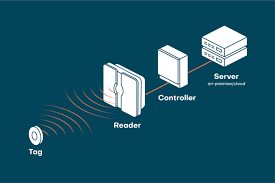
\includegraphics[width=0.5\linewidth]{images/RFID.png}
    \caption{RFID system.}
    \label{fig:RFID}
\end{figure}

\begin{itemize}
    \item \textit{Tags} are small radio frequency labels that store a unique identifier — typically 96 bits in many standards, although other sizes up to 256 bits are possible. They consist of an antenna and a microchip and are attached to the objects we want to identify.

    \item \textit{Readers} are more powerful devices. They transmit a continuous wave or carrier and interrogate tags in their coverage area; they also receive the weak signals backscattered by tags when they reply. 
    \item The \textit{server} is the backend that collects tag IDs, processes them according to application logic and stores the inventory data.
\end{itemize}
RFID systems are used wherever automated identification saves time, reduces errors or enables novel services. You will find them in inventory and logistics, access control, object tracking, library systems, airport baggage handling, assisted living and smart home applications, etc. These systems need to read unique IDs for many objects quickly and often without human intervention.

\begin{figure}[ht]
    \centering
    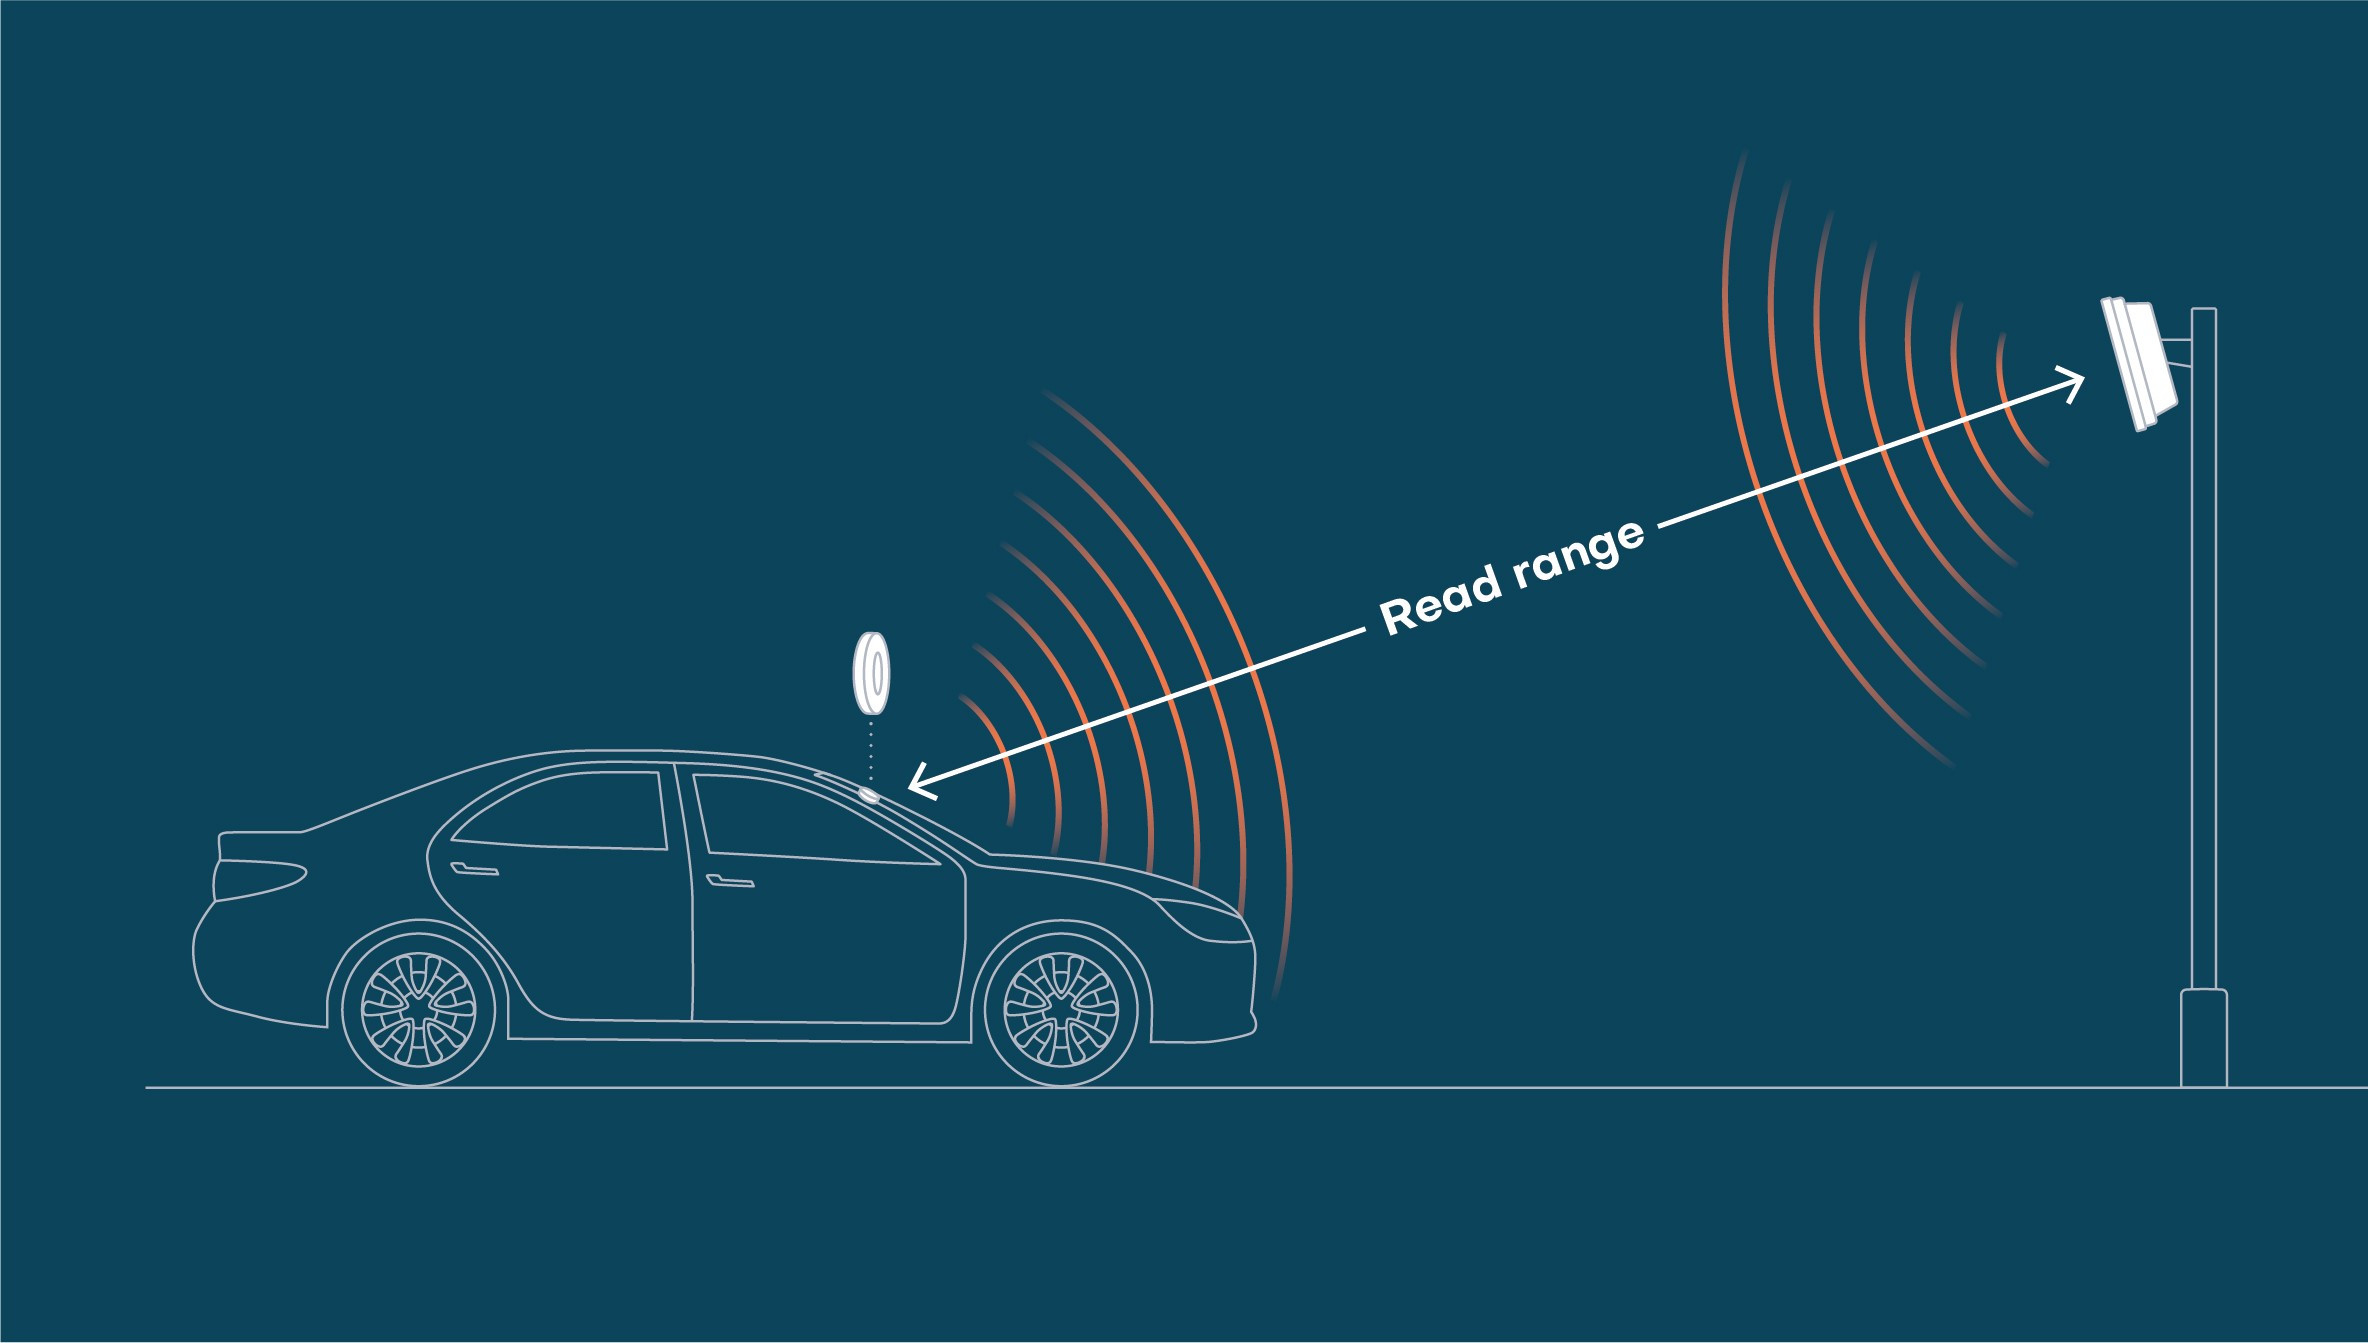
\includegraphics[width=0.5\linewidth]{images/rfid-applications.jpg}
    \caption{RFID application for reading ranges for automatic vehicle identification.}
    \label{fig:rfid-applications}
\end{figure}

\section{RFID communication}
Communication in RFID systems is wireless, between reader and tag. There are two directions of interest: reader-to-tag and tag-to-reader. 
\begin{itemize}
    \item The reader-to-tag link typically carries commands and power.
    \item Tag-to-reader is the way tags report their ID. 
\end{itemize}
Tag-to-tag communication is not allowed because: many tags are passive (have no battery) and their replies are transmitted by \textit{backscattering}\footnote{Backscatter (or backscattering) is the reflection of waves, particles, or signals back to the direction from which they came. Ambient backscatter technology uses existing signals to power and communicate with unpowered sensors.}.

A defining feature of many RFID tags is that they are battery-free. These passive tags harvest power from the reader’s continuous high-power signal. To communicate, the tag does not transmit a fresh radio signal; instead it modifies how it reflects the incoming carrier. The reader senses tiny changes in the reflected wave and decodes the tag’s response.

Because the tag does not generate its own carrier and has very small transmit power, the link is low-rate compared to typical Wi‑Fi connections. Tag-to-reader data rates are often on the order of tens of kilobits per second.

The RFID radio channel has several properties that shape protocol design. It is wireless and shared among all tags in the reader’s range. It is low bitrate and the tags’ replies may overlap in time; when two or more tags reply simultaneously they create a collision from the reader’s perspective. Crucially, passive tags typically cannot hear each other; they have no carrier-sense capability and no collision detection, so the reader must orchestrate which tags speak and when using a protocol to separate them efficiently.

When the reader initiates a reading session, it broadcasts commands to the tags in its field. Tags that match the command or query conditions will reply by backscattering their ID. The reader listens and attempts to decode the returned waveform.

If a single tag replies, the reader can decode its ID and acknowledge it; that tag can then be removed from the set of tags awaiting identification. If multiple tags reply at the same time, their signals mix and the reader is unable to decode individual IDs — we call this a collision. The reader detects a collision and triggers a collision-resolution mechanism, which is the role of the MAC protocol.

\section{MAC protocols}
Several characteristics make the MAC problem unique for RFID. First, there may be a very large number of tags to identify, far more than in typical wireless networks. Second, passive tags cannot initiate communication spontaneously; they wait for the reader’s prompt. Third, tags respond via a backscattered signal that collides when simultaneous. Fourth, tags cannot listen to the channel — there is no carrier sense — and cannot detect collisions. Put together, these constraints force the design of reader-coordinated MAC protocols that aim to separate tag transmissions so that the reader receives one ID at a time.

Researchers have proposed many MAC protocols tailored to RFID. Broadly, we can group them into \textit{sequential protocols} (tree based, Aloha based, etc.) and \textit{concurrent protocols} that try to exploit collisions rather than avoid them. Here we focus only on sequential methods, specifically Tree based and Aloha based.
\begin{itemize}
    \item \textit{Tree-based} methods aim to interactively split the set of tags into smaller subsets until each subset contains a single tag that can be identified. Binary Splitting is a classic example. Query Tree protocols are a related family that use prefix matching and tree traversal. There are improved variants of Query Tree that refine efficiency under different loads.
    \item \textit{Aloha-based} methods borrow ideas from slotted Aloha: the reader defines frames and slots and tags pick a slot to reply. Framed Slotted Aloha is a common approach; some variants are standardized in the EPC Gen2 specification. Tree Slotted Aloha and other modified protocols (for example BSTSA) combine tree and slotted strategies to balance performance across different tag population sizes.
\end{itemize}

\subsection{Binary Splitting}
\textit{Binary Splitting (BS)} is a recursive tree-based approach to singulating tags. The main idea is simple: whenever multiple tags collide, we split the set of colliding tags into two groups and recursively resolve each subgroup until all tags are identified.
Let us walk through how a Binary Splitting session proceeds in practice. 
\begin{enumerate}
    \item Initially every tag participating in the reading has a local counter set to zero. 
    \item The reader issues a generic query that asks tags with counter equal to zero to reply. 
    \item If exactly one tag answers, the reader reads its ID and that tag is considered identified; the reader then broadcasts that fact and the process continues for remaining tags.
    \item If more than one tag answers, the reader detects a collision. On collision, every replying tag generates a random binary digit — either 0 or 1 — and adds that digit to its local counter. The reader then queries again, asking tags with counter equal to zero to reply. This effectively partitions the original set into those tags whose random bit was zero (they keep counter zero) and those whose random bit was one (they increment their counter to one and stay silent for this query). 
    \item If the collision still occurs among the replying tags (the zeros), those tags each again flip a random bit and add it to their counters, further refining the partition.
    \item Meanwhile, tags that are currently silent because their counter is greater than zero increment their counter each time the reader issues a query that they are not eligible to answer. 
    \item The process continues, recursively splitting the colliding group into smaller and smaller subgroups until single-tag responses are obtained. If none or one tag replies, all tags decrement their counter by 1.
\end{enumerate}
An alternative way to view Binary Splitting is that tags generate a random binary tree where each collision makes the algorithm explore two children nodes corresponding to the two possible bit outcomes (see Figure \ref{fig:binary-splitting}). Tags follow a random path down this tree; when a leaf node contains exactly one tag that tag is identified and removed from the active set.

\begin{figure}[ht]
    \centering
    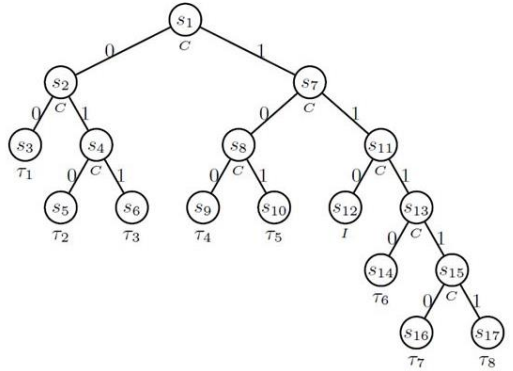
\includegraphics[width=0.6\linewidth]{images/binary-splitting.png}
    \caption{Tree representation of Binary Splitting.}
    \label{fig:binary-splitting}
\end{figure}

\begin{Example}{Eight tag binary splitting}{}
Let's name our eight tags $s_1$ through $s_8$. 

Initially every tag has counter $C = 0$. The reader issues a broad query for counter equals zero; all eight reply and we get a collision.

Now each of the eight tags picks a random bit. Suppose $s_1$, $s_2$ and $s_3$ pick 0 and keep $C=0$; $s_4$, $s_5$, $s_6$, $s_7$ and $s_8$ pick 1 and set $C=1$. The next reader query asks only tags with $C=0$ to reply, so $s_1$, $s_2$ and $s_3$ respond and collide.

Because $s_1$–$s_3$ collide, each of them now picks a fresh random bit and adds it to its counter. Suppose $s_1$ picks 0 (still $C=0$), $s_2$ picks 1 ($C$ becomes 1), $s_3$ picks 0 ($C$ stays 0). The reader queries for $C=0$ again and hears $s_1$ and $s_3$; if they collide again we continue splitting; if only one of them replies we identify it. Meanwhile the silent tags ($s_4$–$s_8$ and eventually $s_2$) wait and increment their counters on each query.

This recursive splitting continues until each group contains only one tag, and all IDs are collected.
\end{Example}

\subsection{Query Tree}
\textit{Query Tree (QT)} protocols use the binary structure of the tag's ID instead of randomized splitting. Each tag has a fixed binary ID. The reader issues queries that are simply binary strings (prefixes). Only tags whose ID begins with the transmitted prefix respond.

\begin{enumerate}
    \item Start by asking the NULL prefix, meaning "everyone reply." 
    \item If a collision occurs, the reader extends the prefix by one bit and re-queries. For example the reader will try prefix "\texttt{0}" and prefix "\texttt{1}". 
    \item If prefix "\texttt{0}" still collides, the reader will try "\texttt{00}" and "\texttt{01}" and so on. 
\end{enumerate}
This procedure traverses an implicit binary tree of all possible IDs: leaves contain either a single matching tag (readable) or none (idle), while internal nodes correspond to collisions that must be split further.

This approach is deterministic in the sense that tags don't generate random bits; the split is guided by actual ID bits. It works well when IDs are uniformly distributed because the tree tends to balance itself, splitting the population roughly in half at each bit expansion. In that uniform-ID case the Query Tree and Binary Splitting produce very similar trees and comparable performance, which is why the literature often compares them directly.

\begin{Example}{Query tree}{}
Suppose three tags have IDs \texttt{0100}, \texttt{0111} and \texttt{1010}. 

\noindent
\begin{minipage}[c]{0.65\textwidth}
The reader starts with the empty prefix and all three reply, causing a collision. The reader then queries prefix "\texttt{0}" and prefix "\texttt{1}". Prefix "\texttt{1}" matches only \texttt{1010}, so \texttt{1010} replies alone and is readable; the reader reads it. Prefix "\texttt{0}" matches \texttt{0100} and \texttt{0111}; they collide so the reader lengthens the prefix to "\texttt{00}" and "\texttt{01}". The prefix "\texttt{00}" is idle, so the reader tries "\texttt{01}," which causes a collision. Finally we come to the prefix "\texttt{010}" which only matches \texttt{0100} (readable) and the prefix "\texttt{011}" which only matches \texttt{0111} (readable).
\end{minipage}
\hfill
\begin{minipage}[c]{0.30\textwidth}
    \centering
    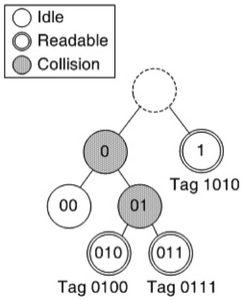
\includegraphics[width=1\textwidth]{images/query-tree-ex.png}
    %\captionsetup{hypcap=false}
    %\captionof{figure}{Query tree.}
    \label{fig:query-tree}
\end{minipage}
\end{Example}

\subsection{Performance of tree protocols}
A simple performance metric is system efficiency, defined as the ratio of successful single-tag responses to the total number of queries the reader sends. Denote by $n$ the number of successful single responses (which equals the number of tags to identify) and by $q$ the total number of queries sent during the identification. Then system efficiency is
\begin{equation*}
    SE = \frac{n}{q}
\end{equation*}
An ideal protocol would have $SE = 1$, meaning every query yields exactly one readable tag and the reader only sends $n$ queries for $n$ tags. In practice, RFIDs face collisions and idle queries, so SE is far below 1. We therefore care about minimizing $q$ for a given $n$.

To estimate how many queries Binary Splitting requires on average to identify $n$ tags, we can write a recursion for the expected total number of queries, which I will call $BS_{tot}(n)$. 
\begin{itemize}
    \item For $n \leq 1$, the protocol needs only one query: the reader asks the broad question and either hears nothing ($n=0$) or hears a single readable tag ($n=1$). So $BS_{tot}(0) = 1$ and $BS_{tot}(1) = 1$.
    \item For $n > 1$, after the first query we always get a collision and must split the set into two subsets. Each tag independently goes left or right with probability $1/2$, so the number of tags $k$ on the left follows a binomial distribution. The expected total queries satisfy
    \[BS_{tot}(n)=
    \begin{cases}
        1, & n \leq 1, \\[6pt]
        1+\displaystyle\sum_{k=0}^n \binom{n}{k}
            \left(\frac{1}{2}\right)^k
            \left(1-\frac{1}{2}\right)^{n-k}
            \bigl(BS_{tot}(k)+BS_{tot}(n-k)\bigr), & n > 1.
    \end{cases}
    \]
    
This equation reads naturally: we pay one query for the root node, then we add the expected cost of resolving the left and right subtrees, averaged over all possible splits (the binomial coefficients give the probability of each split). Because left and right are symmetric you can also collapse the sum to obtain that the fraction of queries that actually return a single readable tag converges to about 0.38, meaning only 38\% of reader queries produce useful, single-tag responses. The remaining 62\% are spent exploring internal tree nodes (collisions) or probing empty branches (idle queries).
\end{itemize}

\subsection{Framed Slotted Aloha}
In \textit{Framed Slotted Aloha (FSA)} the time is divided into slots and each slot is long enough for a tag to transmit its ID. A frame is just a group of consecutive slots. 
\begin{enumerate}
    \item When the reader starts a frame it tells tags how many slots the frame contains. 
    \item Each tag picks one slot at random and transmits in that slot. 
    \item If exactly one tag transmits in a slot the reader hears a readable ID. 
    \item If two or more pick the same slot their backscattered responses collide and the reader cannot decode them. Empty slots happen when no tag picks a given slot.
    \item The process repeats itself until all tags are identified.
\end{enumerate}

\begin{Example}{Framed Slotted Alhoa}{}
Suppose the reader uses 6 slots and, after tags choose, we end up with 3 slots that produced readable single-tag responses and 3 slots that were collision slots. 

\begin{minipage}{\textwidth}
    \centering
    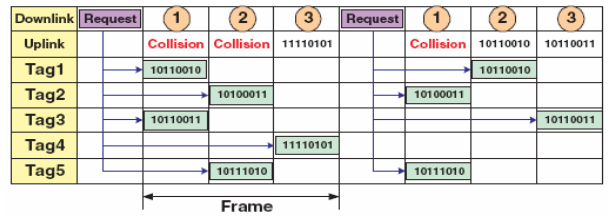
\includegraphics[width=0.7\textwidth]{images/framed-slotted-aloha-ex.png}
    %\captionsetup{hypcap=false}
    %\captionof{figure}{Query tree.}
    \label{fig:framed-slotted-aloha-ex}
\end{minipage}\\

The simple system efficiency measured as 
\begin{equation*}
    \frac{\# identifications}{\# slots} = \frac{3}{6} = 50\%
\end{equation*}
That toy example is optimistic; when you analyze expected behavior for large $n$ the results change.
\end{Example}

For large numbers of tags, average performance is maximized when the frame length $N$ is tuned to match the number of active tags $n$. Intuitively, if you choose too many slots most slots are empty; choose too few and there are too many collisions. For large $n$ the best average successful identifications is about 37\%. Roughly 63\% of slots are wasted (collisions or empties).

\subsubsection{Transmission Time Model}
\textit{EPC Gen2}, the widely adopted commercial standard for passive RFID (Class 1 Gen2), is based on Framed Slotted Aloha. The standard adds practical machinery to improve performance: it defines explicit rules for how the reader adapts frame length based on observed collisions, successful reads and empty slots, and it specifies the low-level timing behavior necessary to compute how long each slot lasts.

Since Gen2 provides a transmission time model, we can translate slot-based metrics into absolute time costs, as illustrated in Figure \ref{fig:epc-gen2}. The timing model defines several relevant delays. There is a tag reaction time \texttt{R1}, which is the delay between the reader command and when the tag begins its reply. The reader has its own reaction time \texttt{R2}, and the reader also sets a threshold \texttt{RX\_threshold}, the point in time by which it should observe the first bit of a tag transmission to conclude a tag is actually transmitting in this slot.

\begin{figure}[ht]
    \centering
    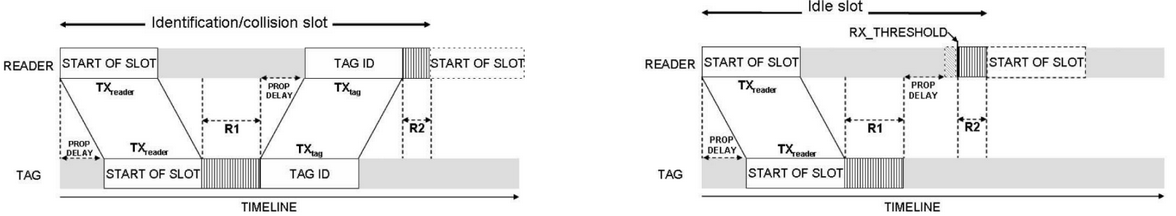
\includegraphics[width=1\linewidth]{images/epc-gen2.png}
    \caption{Transmission time model of EPC Class 1 Gen2.}
    \label{fig:epc-gen2}
\end{figure}

That conversion reveals an important asymmetry: an idle slot — where no tag replies — typically lasts less than a slot with an actual transmission (successful or colliding). In an idle slot the reader detects absence quickly at \texttt{RX\_threshold} and moves on, while collision or successful slots consume the full transmission time.

\subsubsection{Analytical Model}
A classic mathematical abstraction for Framed Slotted Aloha is the balls-and-bins model. Think of $N$ slots as $N$ bins and $n$ tags as $n$ balls. Each tag independently chooses a bin with probability $1/N$. The number of tags that select a given slot follows a binomial distribution. If we are interested in the number of slots that contain exactly $r$ tags, the expected count of such slots is
\begin{equation*}
    s(r) = N\times \binom{n}{r}\left(\frac{1}{N}\right)^r \left(1 - \frac{1}{N}\right)^{n-r}
\end{equation*}
Here $s(r)$ denotes the expected number of slots with exactly $r$ tags, the binomial coefficient $\binom{n}{r}$ counts the ways $r$ tags can occupy the same slot, $\left(\frac{1}{N}\right)^r$ is the probability those $r$ specific tags chose that slot, and $\left(1 - \frac{1}{N}\right)^{n-r}$ is the probability all other $n-r$ tags avoided it. In particular, $s(0)$ is the expected number of idle slots, and $s(1)$ is the expected number of successful identifications within a frame.

From these expressions we can compute key quantities. The expected number of idle slots is
\begin{equation*}
    R_{idle} = N\times \left(1 - \frac{1}{N}\right)^n
\end{equation*}
and the expected number of successful slots (singletons) is
\begin{equation*}
    R_{ident} = n\times \left(1 - \frac{1}{N}\right)^{n-1}
\end{equation*}
The number of collision slots is simply what remains: $R_{coll} = N - R_{idle} - R_{ident}$.

When all slot types have equal duration, the system efficiency measured in slots is $R_{ident} / (R_{idle} + R_{ident} + R_{coll})$, and at the optimal point this equals about 0.36. If we account for different durations (say, idle slots last only a fraction $\beta$ of the full transmission time), we can compute a time-based system efficiency by weighting each class by its duration:
\begin{equation*}
    Time\_SE = \frac{R_{indent}}{\beta R_{idle}+R_{indent}+R_{coll}} = \frac{n\left(1-\frac{1}{N}\right)^{n-1}}{(\beta - 1)N\left(1-\frac{1}{N}\right)^n+N}
\end{equation*}

\begin{figure}[ht]
    \centering
    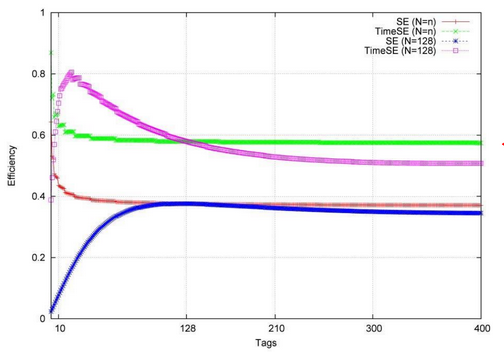
\includegraphics[width=0.7\linewidth]{images/FSA-performance.png}
    \caption{System efficiency and time system efficiency for FSA protocol.}
    \label{fig:FSA-performance}
\end{figure}

\subsection{Tree Slotted Aloha}
\textit{Tree Slotted Aloha (TSA)} tries to get the best of both worlds by adding a tree-structured progression of frames. Instead of using a single frame repeatedly, TSA executes frames following a tree traversal: when a slot collides, a new child frame is issued whose participants are only the tags that collided in that previous slot (see Figure \ref{fig:tree-slotted-aloha}). In other words, collision slots spawn sub-frames devoted solely to resolving that collision.

\begin{figure}[ht]
    \centering
    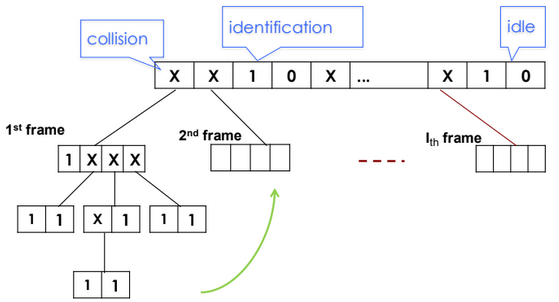
\includegraphics[width=0.7\linewidth]{images/tree-slotted-aloha.png}
    \caption{Tree Slotted Aloha.}
    \label{fig:tree-slotted-aloha}
\end{figure}

Picture the first frame as the root. Each slot in that frame corresponds to a child of the root. If a slot is idle it is a leaf with no tags. If it contains a single tag it is a leaf with a readable tag. If it contains more than one tag (collision), the algorithm issues a child frame that explores that slot’s participants through new slots, each of which becomes a child node in the TSA tree. This process continues until every collision subtree is resolved into readable leaves.

Counting slots in the TSA protocol is equivalent to counting nodes in this dynamic tree. Each node corresponds to a slot, and it is classified as idle, readable, or collision. The TSA total slot count $TSA_{tot}(n)$ for identifying $n$ tags can be written recursively:
\[TSA_{tot}(n)=
    \begin{cases}
        1, & n = 1, \\[6pt]
        n+n\displaystyle\sum_{k=2}^n \binom{n}{k}
            \left(\frac{1}{n}\right)^k
            \left(1-\frac{1}{n}\right)^{n-k}
            \bigl(TSA_{tot}(k)\bigr), & n > 1.
    \end{cases}
\]

When evaluated for large $n$, TSA measured in slots tends to an efficiency $SE_{TSA}$ around 0.43, meaning about 43\% of slot executions yield useful single-tag identifications.

\subsection{Estimating tag population}
Both FSA and TSA rely on choosing a frame length that balances collisions and idle slots. If the frame is too short many collisions occur; if too long many slots are idle. 

The difficulty appears at two levels. First, the very first frame the reader issues needs a good initial size even though it has no prior observations. Conventionally people pick a reasonable default, like 128 slots, but that is often far from optimal when tag populations are very large or very small. Second, during identification, when the reader spawns new frames—especially in Tree Slotted Aloha (TSA)—it must estimate how many tags were involved in the collision that spawned the child frame. Bad estimates lead to inefficient frames, either too many empty slots or too many collisions. So estimating the tag population is central to good protocol performance.

A simple attempt at estimation uses the observed numbers of idle slots, identification slots and collision slots in the last completed frame. If you know those counts and you assume tags chose slots uniformly at random, you can invert the balls-and-bins formulas to obtain an estimate for $n$. The balls-and-bins model says that for a frame with $N$ slots and $n$ tags, the expected number of slots occupied by exactly $r$ tags is
\begin{equation*}
    s(r) = N\times \binom{n}{r}\left(\frac{1}{N}\right)^r \left(1 - \frac{1}{N}\right)^{n-r}
\end{equation*}
In particular, the observed number of singleton slots should be close to the expected value $R_{ident} = n\times \left(1 - \frac{1}{N}\right)^{n-1}$, and the number of idle slots should be close to $R_{idle} = N\times \left(1 - \frac{1}{N}\right)^n$. If we observe triples of counts $\langle c_0,c_1,c_2\rangle$ for idle, singleton and collision slots, we can try to find the value of $n$ that minimizes some distance between the observed triple and the expected triple 
$\langle a_0(n),a_1(n),a_2(n)\rangle$. This is a minimum-distance estimator: search over possible $n$ and pick the one that fits observed data best.

That sounds neat in theory, but there are practical problems. The variance can be huge; the minimum-distance search requires a reasonable range to search; and the upper bound for the search is tricky. A common yet crude bound is $2(c_1 + 2 c_k)$ where $c_1$ is the number of singleton slots and $c_k$ counts the collided slots. For some parameter settings this bound is disastrously small. Suppose there are $n = 5000$ tags, but the reader used an initial frame of $N = 128$. It is extremely likely that every non-empty slot will have multiple tags, so $c_1$, the number of singleton slots, is zero. Plugging $c_1 = 0$ into the bound $2(c_1 + 2 c_k)$ yields roughly 512 as the upper bound for $n$—far smaller than the real $5000$ tags. The estimator then collapses and gives a meaningless result.

When $N$ is small and $n$ is large, the number of occupied slots concentrates on collisions: many tags crowd the same slots and singleton counts vanish. The estimator has almost no signal to distinguish between true $n = 5000$ and some much smaller $n$ that produces very similar $c_0$ and $c_1$ values, so the estimated triples vary surprisingly little as $n$ grows.
Can we do better? 

Instead of relying solely on frame observations to infer $n$, we can use randomized splitting techniques to actively partition the population until the groups are small enough to be estimated accurately or directly identified. This is the intuition behind two complementary solutions: a \textit{dynamic TSA (Dy\_TSA)} and the \textit{Binary Splitting Tree Slotted Aloha (BSTSA)}.

\subsection{Binary Splitting Tree Slotted Aloha}
Binary Splitting uses cheap randomness at the tags to split a large pool into two roughly equal halves; this works well because any large collection of items that randomly split tends to produce subgroups of similar size. TSA, on the other hand, is very good at identifying tags once the participating set size is moderate and a properly sized frame can be used.

BSTSA begins by applying randomized splits to break the initial massive crowd into smaller groups. Once a splitting branch reaches a small group — typically when the left child of a split contains a single tag — BSTSA switches to a Tree Slotted Aloha mode for the remaining sibling subgroups. In other words, use Binary Splitting for coarse partitioning and TSA for the final singulation and identification within each manageable subgroup.

\begin{figure}[ht]
    \centering
    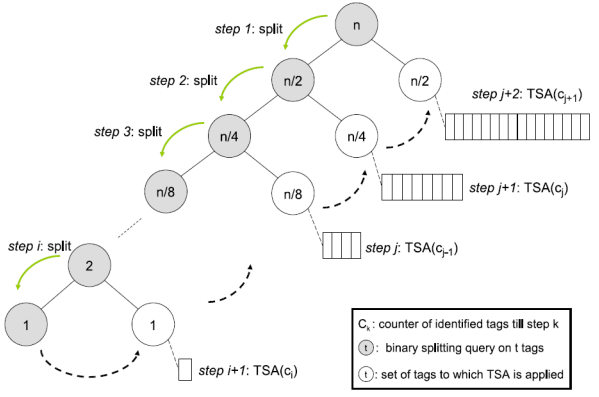
\includegraphics[width=0.8\linewidth]{images/binary-splitting-tree-slotted-aloha.png}
    \caption{Binary Splitting Tree Slotted Aloha.}
    \label{fig:binary-splitting-tree-slotted-aloha}
\end{figure}

This hybrid offers a few practical advantages. First, splitting is cheap from the tag side and helps avoid the pathological case where an initial frame is tiny relative to the population. Second, after partitioning, TSA can adopt close-to-optimal frame sizes for each subgroup because the estimated group sizes are now in a range where balls-and-bins inversion is meaningful. The overall effect is improved time efficiency and reduced latency versus plain TSA or FSA with naive initialization.

\begin{figure}[ht]
    \centering
    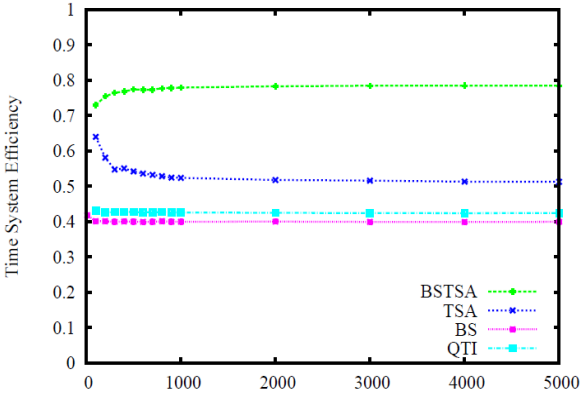
\includegraphics[width=0.6\linewidth]{images/efficency-BSTSA.png}
    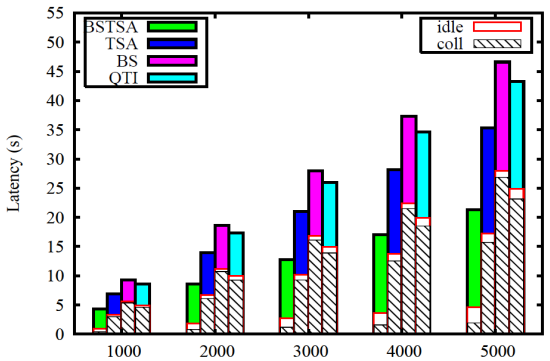
\includegraphics[width=0.6\linewidth]{images/latency-BSTSA.png}
    \caption{Time system efficiency and latency in Binary Splitting Tree Slotted Aloha.}
    \label{fig:efficiency-latency-BSTSA}
\end{figure}